\documentclass[a4paper,english]{article}
\usepackage{graphicx}
\usepackage{listings}
\usepackage{amsmath}
%% Use utf-8 encoding for foreign characters
%%\usepackage[T1]{fontenc}
%%\usepackage[utf8]{inputenc}
%%\usepackage{babel}
%%
%%%% Vector based fonts instead of bitmaps
%%\usepackage{lmodern}
%%
%%%% Useful
%%%\usepackage{fullpage} % Smaller margins
%%\usepackage{enumerate}
%%
%%%% Theorem
%%\usepackage{amsthm}
%%
%%%% More math
%%\usepackage{amsmath}
%%\usepackage{amssymb}
\lstset{
  breaklines=true,
  postbreak=\mbox{{$\hookrightarrow$}\space},
}
%% Document Header
\title{Section6}
\author{Elliott Ashby}
\date{\today}

\begin{document}
    \maketitle
    \section{q1}
        Using the code as suggested, but with a key difference, only printing the values when t is 1 
        or t is 2 allows us to easily obtain the required date at the specified times.
        \lstinputlisting[language=Python]{./q6_1.py}
        Since this code will be used for q2 aswell, different values of dt are considered, to find the wanted values at
        dt is 0.2 simply look at the output below "when dt is 0.2".
        \begin{center}
            when dt is 0.2 and when\\
                RC=1.0, V=0.67232\\
                RC=2.0, V=0.8926258176\\
        \end{center}
    \section{q2}
        The above code also prints the values when dt is 0.1, 0.02 and 0.01.
        \begin{center}
            when dt is 0.1 and when\\
                RC=1.0, V=0.6513215599000001\\
                RC=2.0, V=0.8784233454094308\\
                \medskip
            when dt is 0.02 and when\\
                RC=1.0, V=0.6358303199128829\\
                RC=2.0, V=0.867380444105247\\
                \medskip
            when dt is 0.01 and when\\
                RC=1.0, V=0.6339676587267709\\
                RC=2.0, V=0.8660203251420382\\
        \end{center}
    \section{q3}
    \lstinputlisting[language=Python, lastline=9]{./q6_3.py}  
        Here we modify odestep into a form that takes into account the possible change in gradient of the slope without
        having dt very small. We can do this by taking the average of two gradients like:
        \begin{equation*}
            y(t+\delta t) = y(t) + \frac{1}{2}\left[ \left( \frac{dy}{dt}\right)_{A}+\left( \frac{dy}{dt}\right)_{B^{'}}\right]\delta t
        \end{equation*}
    \section{q4}
        Using the new system yields:
        \begin{center}
            when dt is 0.2 and when\\
                RC=1.0, V=0.6292601568\\
                RC=2.0, V=0.8625519686640395\\
        \end{center}
    \section{q5}
        In order to get more accurate values we can decrease dt until only extremely small changes occur in V.
        In order to implement this, we can simply make a requirement that the previous value of V has to be less
        than a certain magnitude, in this case I chose 1.0e-6 arbritrarily.
        \lstinputlisting[language=Python, firstline=12]{./q6_3.py}
        Here, if both of the V values at t = 1 and t = 2 meet the stopping value, no more values are calculated.
    \section{q6}
        Here we simply alter the code to include g(t) = cos(t) and up the value of tf, then we can plot $\omega$ = 0.5, 1 and 2
        along with the input signal.
        \lstinputlisting[language=Python, lastline=19]{./q6_6.py}
        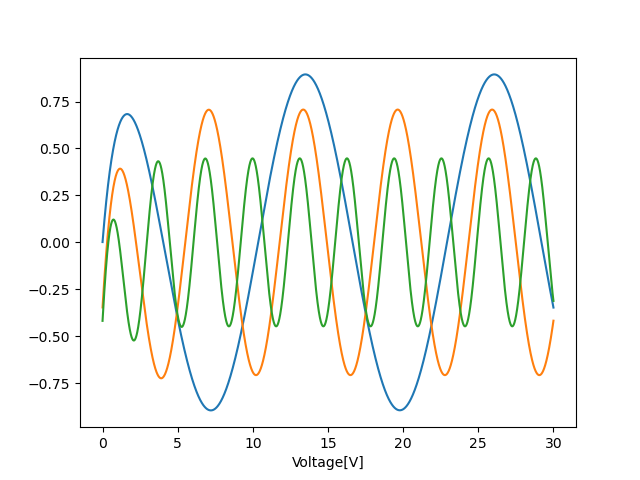
\includegraphics[scale=0.74]{q6_6_t0.png}
    \section{q7}
        We can make plots for increasing values of y in order to inspect their differences.
        \lstinputlisting[language=Python, firstline=22]{./q6_6.py}
        Here we simply count i upwards to 10 (the only reason I used a yield function to play around with generators)
        Then we generate a new plot of all three $\omega$s while substituting the y value for the value of i.
        Here are where y = 0, 5 and 10.
        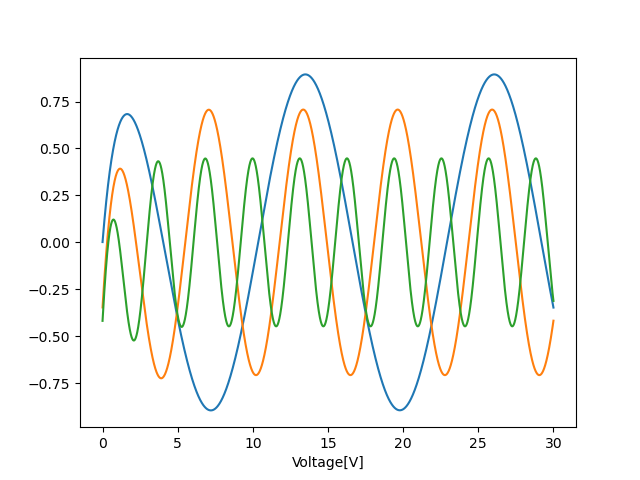
\includegraphics[scale=0.74]{q6_6_t0.png}\\
        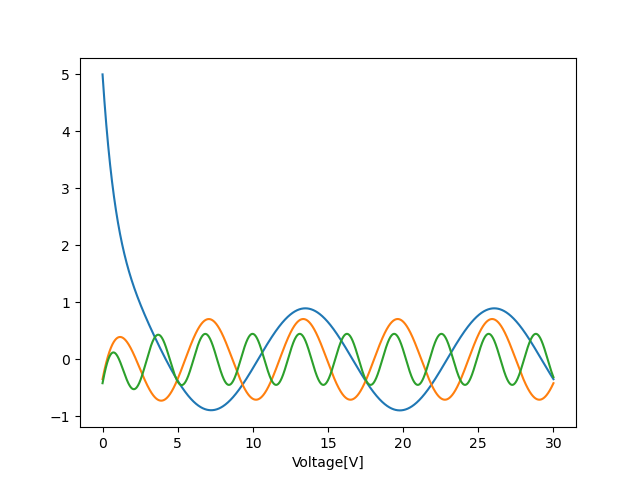
\includegraphics[scale=0.74]{q6_6_t5.png}\\
        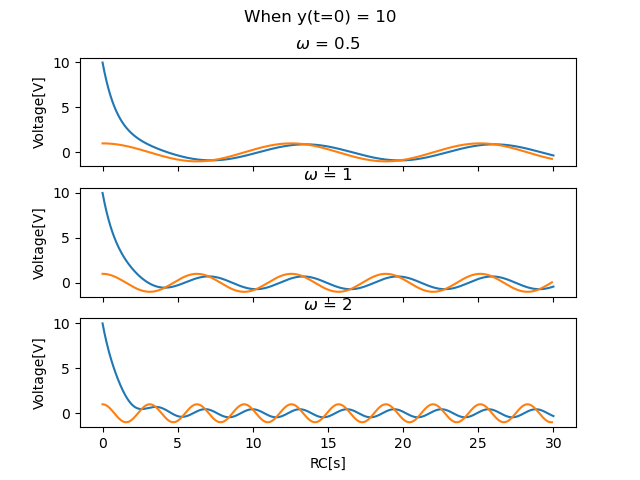
\includegraphics[scale=0.74]{q6_6_t10.png}\\
        We can see here that the y(t=0) value determines the starting value of the curve, meaning, the further away from the average
        value of the curve is is the longer the curve takes to "settle" into it's predicted cosine pattern.
    \section{q8}
        In order to find the amplitude of each value of $\omega$ we can simply print the maximum value of the data set.
        And to find the phase we can cross correlate the input signal and the output signal.
        \begin{center}
            When $\omega$ = 0.5\\
            Amplitude = 0.8944271397260981\\
            Phase difference = 1.096944476599115 rads\\
            \medskip
            When $\omega$ = 1\\
            Amplitude = 0.7071066610319001\\
            Phase difference = 5.045320129800867 rads\\
            \medskip
            When $\omega$ = 2\\
            Amplitude = 0.44721361538056764\\
            Phase difference = 5.42234390436165 rads\\
        \end{center}
        This was done like:
        \lstinputlisting[language=Python, firstline=75]{./q6_6.py}
\end{document}
